%% Creator: Inkscape inkscape 0.92.2, www.inkscape.org
%% PDF/EPS/PS + LaTeX output extension by Johan Engelen, 2010
%% Accompanies image file 'bat1p.eps' (pdf, eps, ps)
%%
%% To include the image in your LaTeX document, write
%%   \input{<filename>.pdf_tex}
%%  instead of
%%   \includegraphics{<filename>.pdf}
%% To scale the image, write
%%   \def\svgwidth{<desired width>}
%%   \input{<filename>.pdf_tex}
%%  instead of
%%   \includegraphics[width=<desired width>]{<filename>.pdf}
%%
%% Images with a different path to the parent latex file can
%% be accessed with the `import' package (which may need to be
%% installed) using
%%   \usepackage{import}
%% in the preamble, and then including the image with
%%   \import{<path to file>}{<filename>.pdf_tex}
%% Alternatively, one can specify
%%   \graphicspath{{<path to file>/}}
%% 
%% For more information, please see info/svg-inkscape on CTAN:
%%   http://tug.ctan.org/tex-archive/info/svg-inkscape
%%
\begingroup%
  \makeatletter%
  \providecommand\color[2][]{%
    \errmessage{(Inkscape) Color is used for the text in Inkscape, but the package 'color.sty' is not loaded}%
    \renewcommand\color[2][]{}%
  }%
  \providecommand\transparent[1]{%
    \errmessage{(Inkscape) Transparency is used (non-zero) for the text in Inkscape, but the package 'transparent.sty' is not loaded}%
    \renewcommand\transparent[1]{}%
  }%
  \providecommand\rotatebox[2]{#2}%
  \ifx\svgwidth\undefined%
    \setlength{\unitlength}{395.9999901bp}%
    \ifx\svgscale\undefined%
      \relax%
    \else%
      \setlength{\unitlength}{\unitlength * \real{\svgscale}}%
    \fi%
  \else%
    \setlength{\unitlength}{\svgwidth}%
  \fi%
  \global\let\svgwidth\undefined%
  \global\let\svgscale\undefined%
  \makeatother%
  \begin{picture}(1,0.833939)%
    \put(0,0){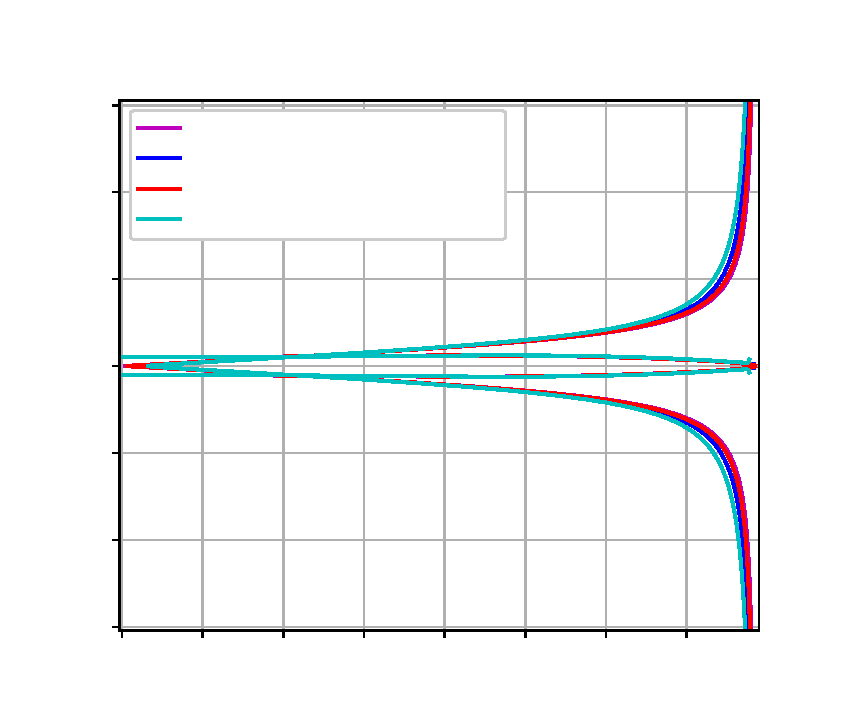
\includegraphics[width=\unitlength]{imagesbat/bat1p.eps}}%
    \put(0.10764293,0.05){\color[rgb]{0,0,0}\makebox(0,0)[lb]{\smash{0.0}}}%
    \put(0.20539672,0.05){\color[rgb]{0,0,0}\makebox(0,0)[lb]{\smash{0.2}}}%
    \put(0.30314899,0.05){\color[rgb]{0,0,0}\makebox(0,0)[lb]{\smash{0.4}}}%
    \put(0.40090404,0.05){\color[rgb]{0,0,0}\makebox(0,0)[lb]{\smash{0.6}}}%
    \put(0.49865657,0.05){\color[rgb]{0,0,0}\makebox(0,0)[lb]{\smash{0.8}}}%
    \put(0.59641162,0.05){\color[rgb]{0,0,0}\makebox(0,0)[lb]{\smash{1.0}}}%
    \put(0.69416414,0.05){\color[rgb]{0,0,0}\makebox(0,0)[lb]{\smash{1.2}}}%
    \put(0.79191667,0.05){\color[rgb]{0,0,0}\makebox(0,0)[lb]{\smash{1.4}}}%
    \put(0.05,0.08659355){\color[rgb]{0,0,0}\makebox(0,0)[lb]{\smash{-15}}}%
    \put(0.05,0.19199405){\color[rgb]{0,0,0}\makebox(0,0)[lb]{\smash{-10}}}%
    \put(0.07,0.29739355){\color[rgb]{0,0,0}\makebox(0,0)[lb]{\smash{-5}}}%
    \put(0.09,0.40279506){\color[rgb]{0,0,0}\makebox(0,0)[lb]{\smash{0}}}%
    \put(0.085,0.50819405){\color[rgb]{0,0,0}\makebox(0,0)[lb]{\smash{5}}}%
    \put(0.065,0.61359557){\color[rgb]{0,0,0}\makebox(0,0)[lb]{\smash{10}}}%
    \put(0.067,0.71899456){\color[rgb]{0,0,0}\makebox(0,0)[lb]{\smash{15}}}%
    \put(0.03065808,0.39910819){\color[rgb]{0,0,0}\rotatebox{90}{\makebox(0,0)[lb]{\smash{$\hat{\omega_0}$}}}}%
    \put(0.21843434,0.69249708){\color[rgb]{0,0,0}\makebox(0,0)[lb]{\smash{\footnotesize $R=1.0m, r_2=1cm$}}}%
    \put(0.21843434,0.65544658){\color[rgb]{0,0,0}\makebox(0,0)[lb]{\smash{\footnotesize$R=1.0m, r_2=5cm$}}}%
    \put(0.21843434,0.61839607){\color[rgb]{0,0,0}\makebox(0,0)[lb]{\smash{\footnotesize$R=0.5m, r_2=1cm $}}}%
    \put(0.21843434,0.58134557){\color[rgb]{0,0,0}\makebox(0,0)[lb]{\smash{\footnotesize$R=0.5m, r_2=5cm $}}}%
    \put(0.42,0.0){\color[rgb]{0,0,0}\makebox(0,0)[lb]{\smash{ $\theta_0 (rad)$}}}%
    \put(0.49865657,0.25){\color[rgb]{0,0,0}\makebox(0,0)[lb]{\smash{stable}}}%
    \put(0.49865657,0.5){\color[rgb]{0,0,0}\makebox(0,0)[lb]{\smash{stable}}}%
    \put(0.6,0.40279506){\color[rgb]{0,0,0}\makebox(0,0)[lb]{\smash{instable}}}%
  \end{picture}%
\endgroup%
